% !TEX program = lualatex
% =====================================================================================
%  PÔSTER 60 x 90 cm -- modelo "Mostra UFMG / DCC" (Projeto Orientado em Computação)
%  Compilador: LuaLaTeX (Menu > Settings > Compiler).  Fontes do modelo: Tomorrow (títulos)
%  e Titillium Web (texto), instaladas no servidor do Overleaf do DCC.
%  O fundo (borda, faixa vermelha, subtítulo e rodapé com QR code e logos) vem de
%  fundo_poster.pdf, que é o próprio modelo oficial sem o texto do título; a faixa vermelha
%  e o subtítulo foram subidos 1,72 cm, acompanhando o título mais compacto.
%
%  COMO EDITAR
%   - Título: \TituloLinhaUm e \TituloLinhaDois (duas linhas, como no modelo). Cada linha
%     encolhe sozinha se passar de 54 cm de largura.
%   - Estrutura: Introdução, Metodologia e Base de dados resultante (coluna esquerda);
%     Resultados, Conclusões e Limitações e trabalhos futuros (coluna direita).
%   - Autores: \Autores.
%   - O conteúdo fica em duas colunas, \begin{coluna}{x} ... \end{coluna}, lidas de cima
%     para baixo: primeiro a da esquerda, depois a da direita.
%   - Dentro de cada coluna, as seções são separadas por \proxima. O espaço entre elas se
%     ajusta sozinho para a coluna ir de \Ytopo a \Ybase (em cm, a partir do topo).
%     Para trocar a ordem, basta mover a seção. Se uma coluna ficar cheia demais, o log
%     mostra "Overfull \vbox": encurte um texto ou diminua um gráfico.
%   - O texto é justificado, com hifenização em português.
%   - Gráficos: os números estão no próprio código (procure "coordinates"). Fonte dos
%     números: outputs/tables/*.csv (coleta de 15/11/2026) e relatorio.tex.
%   - \gradetrue (no preâmbulo) desenha uma grade de 1 cm para ajudar a posicionar.
% =====================================================================================
\documentclass{article}
\usepackage[paperwidth=60cm,paperheight=90cm,margin=0cm]{geometry}
\usepackage{iftex}
\usepackage{amsmath}
\usepackage{fontspec}
\IfFileExists{brazilian.ldf}{\usepackage[brazilian]{babel}}{%
  \IfFileExists{portuges.ldf}{\usepackage[portuges]{babel}}{}}
\IfFileExists{lualatex-math.sty}{\usepackage{unicode-math}\newcommand\temmath{1}}{}
\usepackage{anyfontsize}
\usepackage{graphicx}
\usepackage{adjustbox}
\usepackage{xcolor}
\usepackage{eso-pic}
\usepackage[absolute,overlay]{textpos}
\usepackage{tikz}
\usetikzlibrary{arrows.meta,calc,positioning}
\usepackage{pgfplots}
\pgfplotsset{compat=1.18}
\usepackage{tcolorbox}
\usepackage{enumitem}
\usepackage{tabularx,array}
\usepackage{ragged2e}
\usepackage{csquotes}
\usepackage{xspace}

% ------------------------------------------------------------------ fontes do modelo
% No Overleaf do DCC, Titillium Web e Tomorrow estão instaladas. Fora dele, o pôster usa
% fontes parecidas do TeX Live (Fira Sans e Montserrat) só para não quebrar a compilação.
\IfFontExistsTF{TitilliumWeb-Regular.ttf}{%
  \setmainfont{TitilliumWeb}[Extension=.ttf, UprightFont=*-Regular, BoldFont=*-Bold,
    ItalicFont=*-Italic, BoldItalicFont=*-BoldItalic]
  \newfontfamily\semib{TitilliumWeb-SemiBold.ttf}%
}{\IfFontExistsTF{FiraSans-Regular.otf}{%
  \setmainfont{FiraSans}[Extension=.otf, UprightFont=*-Regular, BoldFont=*-Bold,
    ItalicFont=*-Italic, BoldItalicFont=*-BoldItalic]
  \newfontfamily\semib{FiraSans-SemiBold.otf}%
}{\setmainfont{Carlito}\newfontfamily\semib{Carlito}[UprightFont=* Bold]}}
\IfFontExistsTF{Tomorrow-Bold.ttf}{%
  \newfontfamily\tomorrow{Tomorrow-Bold.ttf}%
}{\IfFontExistsTF{Montserrat-ExtraBold.otf}{\newfontfamily\tomorrow{Montserrat-ExtraBold.otf}}%
  {\newfontfamily\tomorrow{Inter Display Black}}}
\ifdefined\temmath\IfFontExistsTF{FiraMath-Regular.otf}{\setmathfont{FiraMath-Regular.otf}}{\setmathfont{Latin Modern Math}}\fi

% ------------------------------------------------------------------ cores do modelo
\definecolor{vermelho}{RGB}{201,12,12}     % a faixa e a borda do modelo
\definecolor{preto}{RGB}{20,20,20}
\definecolor{cinzaescuro}{RGB}{77,77,77}
\definecolor{cinzamedio}{RGB}{150,150,150}
\definecolor{cinzaclaro}{RGB}{242,242,242}

% ------------------------------------------------------------------ fundo (modelo oficial)
\AddToShipoutPictureBG*{\AtPageLowerLeft{%
  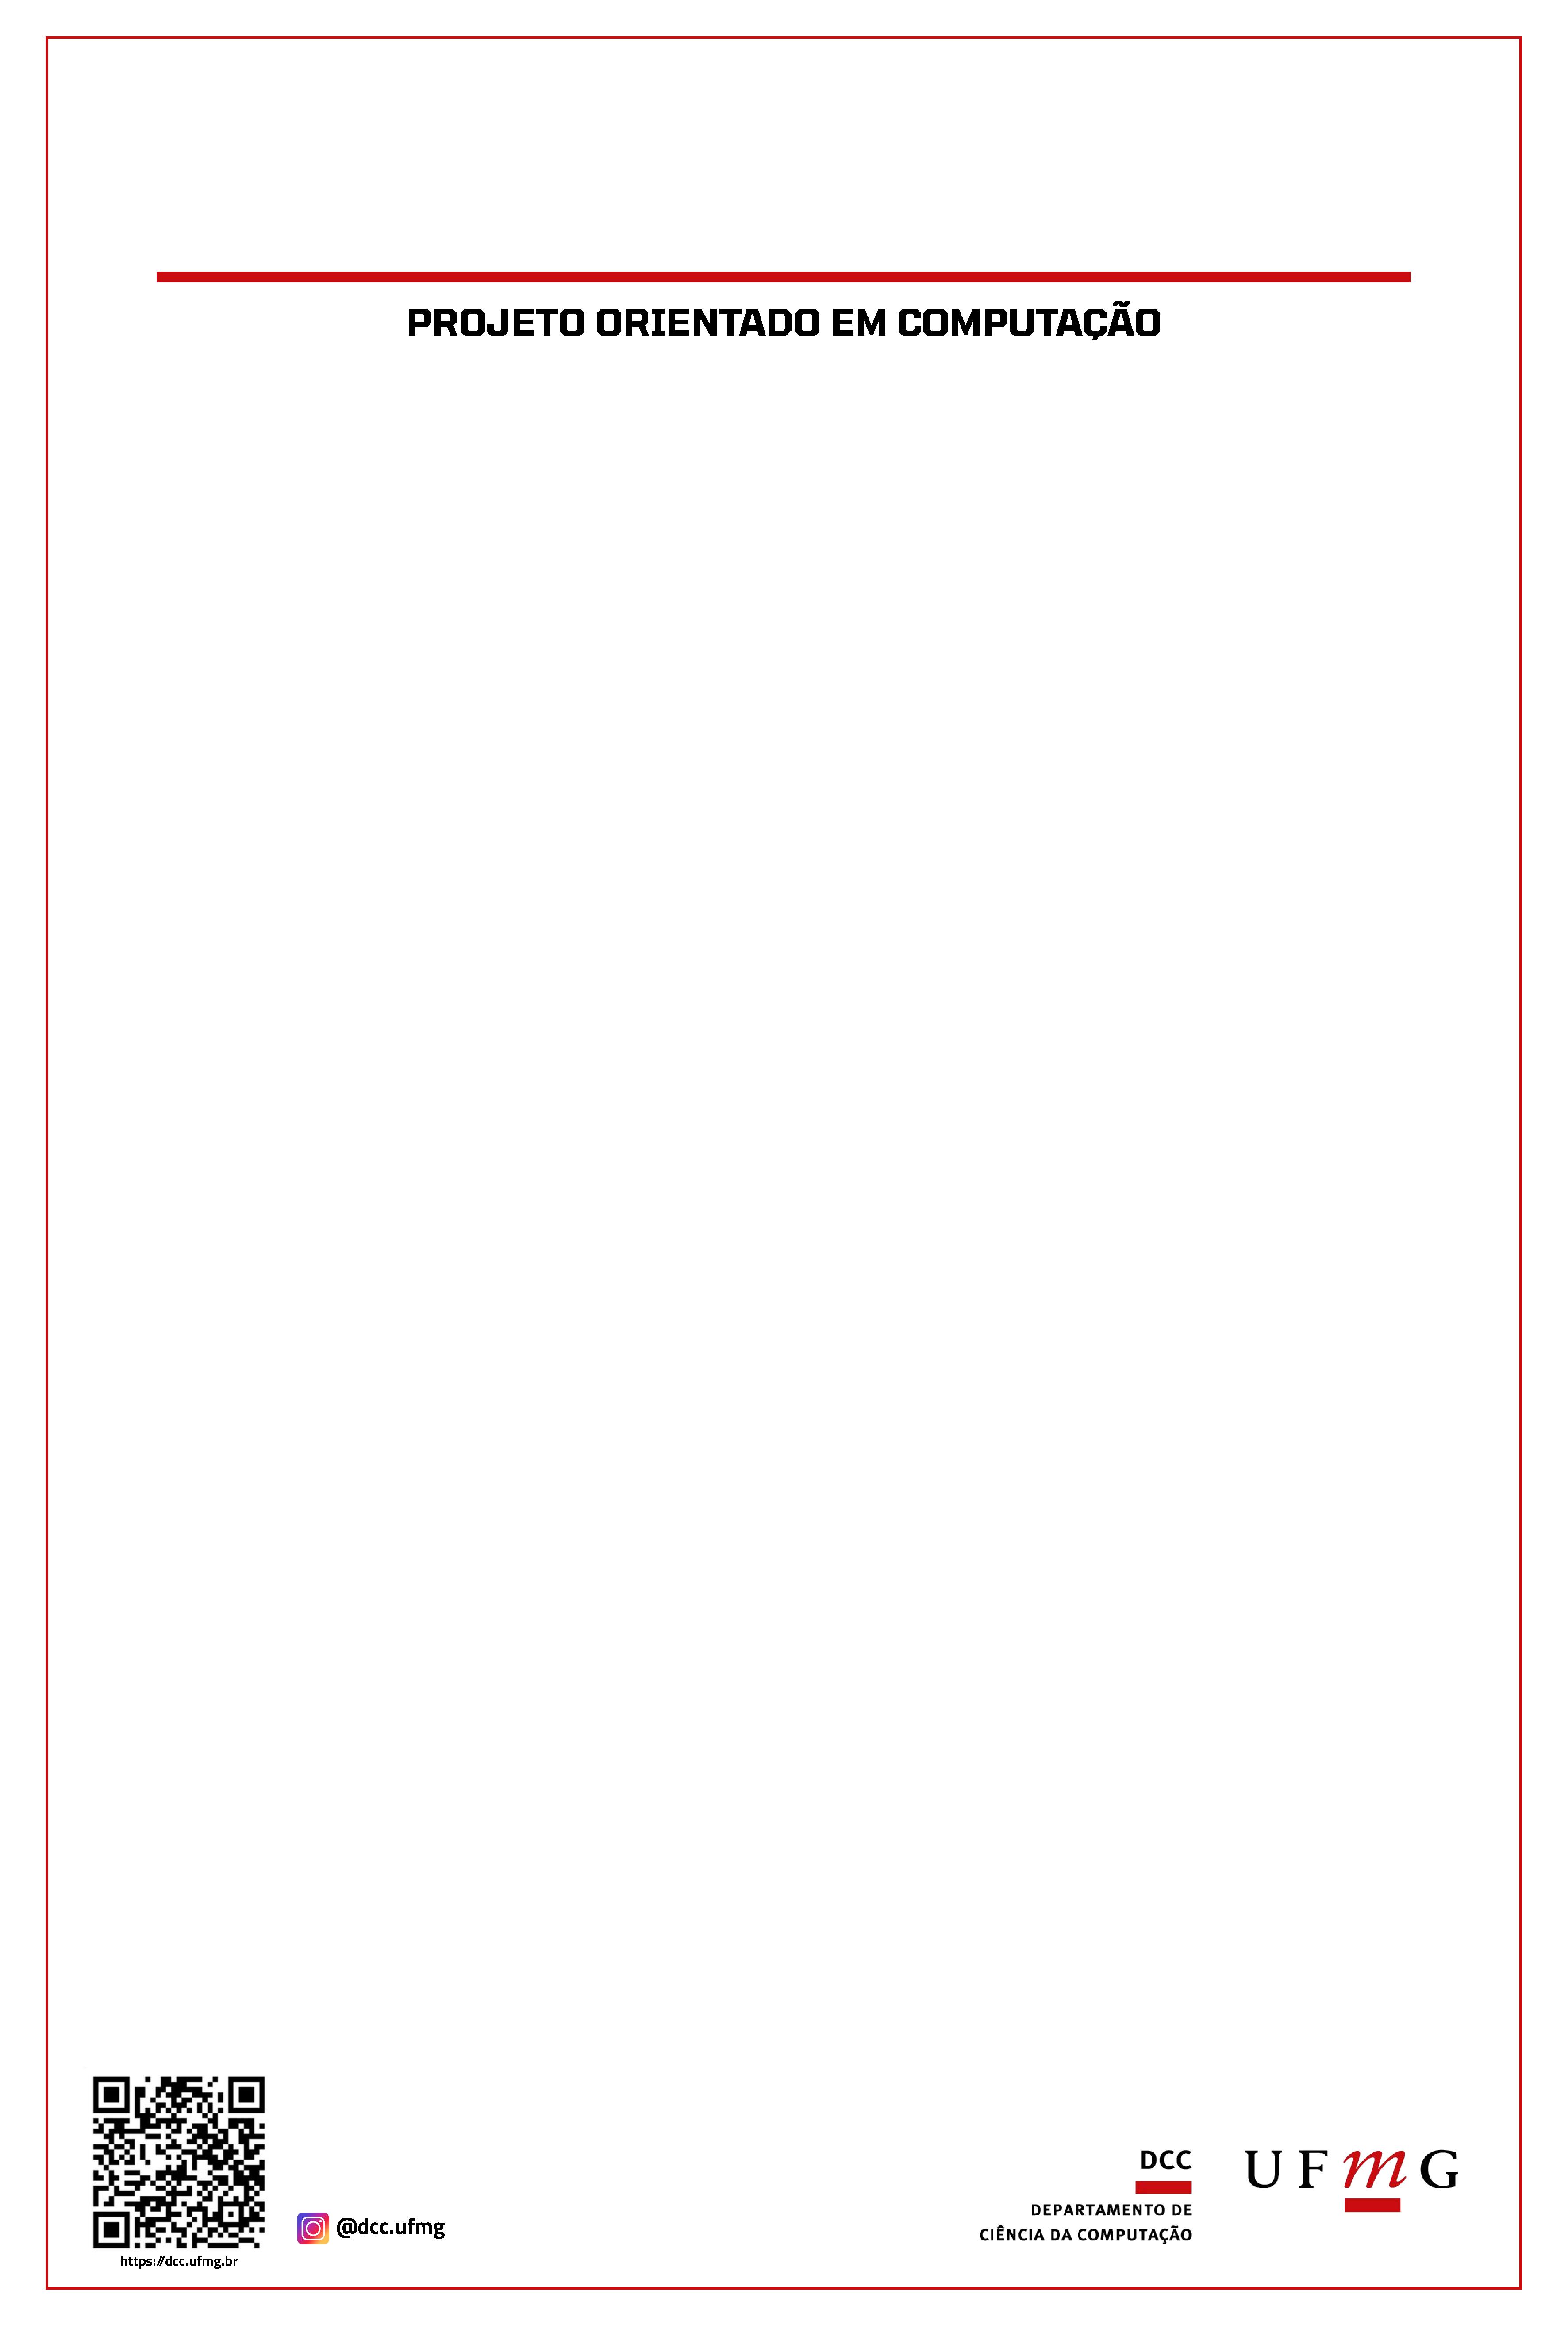
\includegraphics[width=\paperwidth,height=\paperheight]{fundo_poster.pdf}}}

\newcommand{\TituloLinhaUm}{CONTEÚDO SENSÍVEL EM ROMANCES NO BRASIL:}
\newcommand{\TituloLinhaDois}{CONSTRUÇÃO DE UMA BASE VIA FOLKSONOMIA}
\newcommand{\Autores}{Gabriella de Lima Araujo \quad\textcolor{vermelho}{\textbullet}\quad
  Orientadora: Michele Amaral Brandão}

% ------------------------------------------------------------------ estilo do texto
\setlength{\TPHorizModule}{1cm}
\setlength{\TPVertModule}{1cm}
\setlength{\parindent}{0pt}
\setlength{\parskip}{0.3em}
\newcommand{\corpo}{\fontsize{26}{32}\selectfont}
\newcommand{\pequeno}{\fontsize{21}{26}\selectfont}
\newcommand{\minusculo}{\fontsize{16}{20}\selectfont}
\newcommand{\pp}{\,p.p.\@\xspace}

% título de seção: Tomorrow em caixa alta, com a barra vermelha dos logos DCC/UFMG
\newcommand{\secao}[1]{%
  {\tomorrow\fontsize{37}{40}\selectfont\color{preto}#1\par}%
  \vspace{0.08cm}{\color{vermelho}\rule{3.8cm}{0.28cm}}\par\vspace{0.18cm}}
\newcommand{\rotulo}[1]{{\tomorrow\fontsize{23}{28}\selectfont\color{vermelho}#1}}

\setlist[itemize]{label={\textcolor{vermelho}{\rule[0.13em]{0.42em}{0.42em}}},
  leftmargin=1.15em, labelsep=0.55em, itemsep=0.32em, topsep=0.25em, parsep=0pt, partopsep=0pt}

\newtcolorbox{destaque}[1][]{colback=cinzaclaro, colframe=vermelho, boxrule=0pt,
  leftrule=0.45cm, arc=0pt, outer arc=0pt, left=0.9cm, right=0.9cm, top=0.7cm, bottom=0.7cm,
  boxsep=0pt, before skip=0.2cm, after skip=0cm, halign=justify, #1}

% ------------------------------------------------------------------ gráficos
\pgfplotsset{
  /pgf/number format/use comma,
  every axis/.append style={font=\fontsize{24}{28}\selectfont, line width=1.6pt,
    tick style={line width=1.4pt, color=cinzaescuro}, axis line style={cinzaescuro}},
  every tick label/.append style={font=\fontsize{24}{28}\selectfont},
  legend style={font=\fontsize{23}{28}\selectfont, draw=none, fill=none},
}

% prevalência de um eixo (quatro lado a lado, alinhados pela base para não passar de \Ybase)
\newcommand{\prev}[2]{\begin{minipage}[b]{0.25\linewidth}\centering
  {\tomorrow\fontsize{40}{44}\selectfont\color{vermelho}#1}\\[0.1cm]
  {\pequeno\color{preto}#2}\end{minipage}}
% frase-achado acima de cada gráfico: \achado{texto}
\newcommand{\achado}[1]{{\semib\fontsize{27}{33}\selectfont\color{preto}#1\par}\vspace{0.25cm}}
% etapa da metodologia: \etapa{título}{texto}
\newcommand{\etapa}[2]{%
  \vspace{0.15cm}{\color{cinzamedio!60}\rule{\linewidth}{1.2pt}}\par\vspace{0.1cm}
  {\rotulo{#1}}\par\vspace{0.1cm}
  {\fontsize{25}{31}\selectfont #2\par}}
% linha do rótulo: \nivel{nome}{n}{significado}
\newcommand{\nivel}[3]{%
  \noindent\makebox[8.6cm][l]{\rotulo{#1}}%
  \makebox[1.8cm][r]{\semib #2}\hspace{0.6cm}%
  \parbox[t]{\dimexpr\linewidth-11.3cm\relax}{\raggedright\pequeno\color{cinzaescuro}#3}\par\vspace{0.25cm}}
% fontes das caixas do diagrama do pipeline
\newcommand{\cxnome}{\tomorrow\fontsize{21}{24}\selectfont\color{vermelho}}
\newcommand{\cxdet}{\fontsize{17.5}{21}\selectfont\color{preto}}
% conteúdo de uma caixa: \cx{NOME}{detalhe}  (o \par dentro do grupo fixa a entrelinha)
\newcommand{\cx}[2]{{\cxnome #1\par}\vspace{0.1cm}{\cxdet #2\par}}

% ------------------------------------------------------------------ colunas
\newcommand{\Ytopo}{15.2}         % topo das colunas (cm, a partir do topo da página)
\newcommand{\Ybase}{77.6}         % base das colunas (diminua para subir o fim das colunas; QR code em 79,4 cm)
\newcommand{\LarguraColuna}{26.2}  % colunas em x = 3 e x = 30,8
\newenvironment{coluna}[1]{% #1 = x da coluna, em cm
  \begin{textblock}{\LarguraColuna}(#1,\Ytopo)%
  \begin{minipage}[t][\dimexpr\Ybase cm-\Ytopo cm\relax][s]{\LarguraColuna cm}%
  \corpo\setlength{\emergencystretch}{1.5em}}%
  {\par\end{minipage}\end{textblock}}
\newcommand{\proxima}{\par\vfill}  % separa as seções de uma coluna

% bloco de conteúdo: \begin{bloco}{largura}{x}{y} ... \end{bloco}  (em cm, a partir do canto
% superior esquerdo da página)
\newenvironment{bloco}[3]{\begin{textblock}{#1}(#2,#3)\corpo\setlength{\emergencystretch}{1.5em}}{\end{textblock}}

% grade auxiliar de 1 cm (true = desenha)
\newif\ifgrade \gradefalse
\newcommand{\grade}{\ifgrade\begin{textblock}{60}(0,0)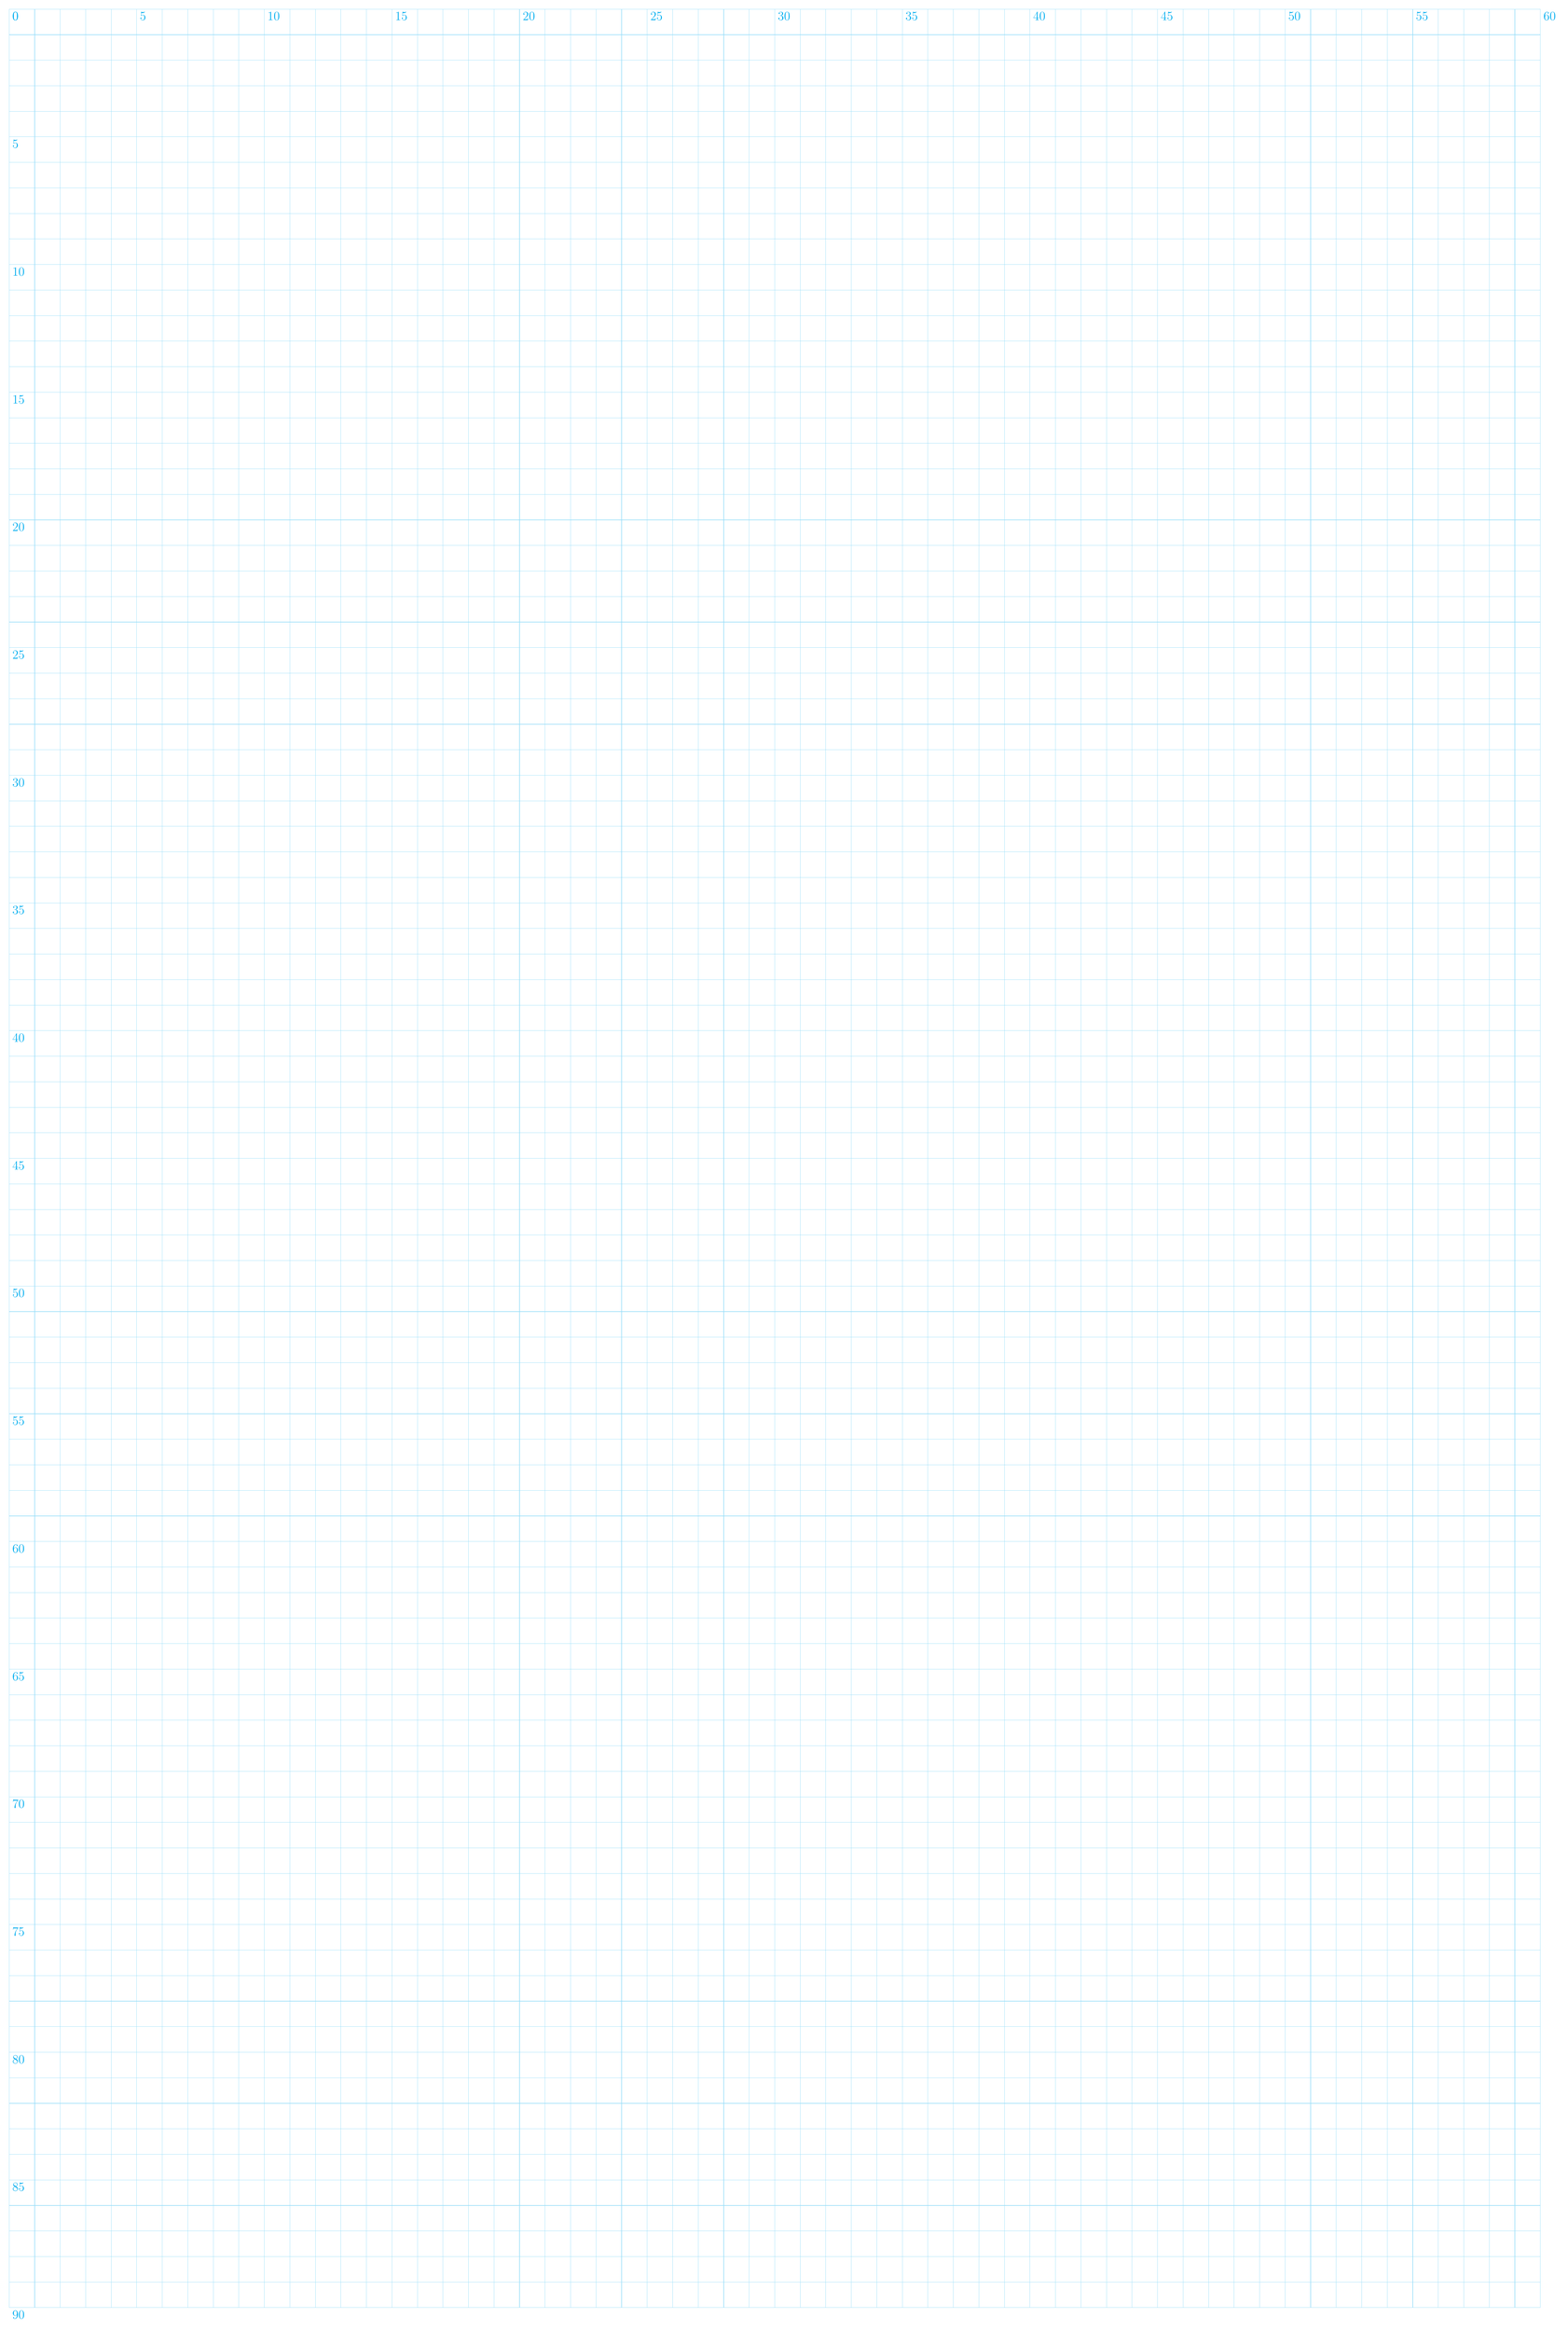
\begin{tikzpicture}[x=1cm,y=1cm]
  \draw[cyan!40,line width=0.4pt] (0,0) grid (60,-90);
  \foreach \i in {0,5,...,60} \node[cyan,anchor=north west,font=\fontsize{14}{14}\selectfont] at (\i,0) {\i};
  \foreach \j in {0,5,...,90} \node[cyan,anchor=north west,font=\fontsize{14}{14}\selectfont] at (0,-\j) {\j};
  \end{tikzpicture}\end{textblock}\fi}

% =====================================================================================
\begin{document}
\pagestyle{empty}
\corpo
\grade

% ---------------------------------------------------------------- título (2 linhas)
% Cada linha é reduzida automaticamente se passar de 54 cm de largura (adjustbox), então o
% título nunca invade a borda. Para subir ou descer o título, mude o 3.4 (cm a partir do topo).
\begin{textblock}{56}(2,3.4)
  \centering{\tomorrow\fontsize{58}{80}\selectfont\color{preto}%
  \adjustbox{max width=54cm}{\TituloLinhaUm}\\
  \adjustbox{max width=54cm}{\TituloLinhaDois}\par}
\end{textblock}

% ---------------------------------------------------------------- autores
\begin{textblock}{54}(3,13.53)
  \centering{\semib\fontsize{32}{38}\selectfont\color{cinzaescuro}\Autores\par}
\end{textblock}

% =====================================================================================
%  COLUNA DA ESQUERDA: Introdução -> Metodologia -> Resultados (1: a base)
% =====================================================================================
\begin{coluna}{3}
% ---------------- 1. introdução: contexto, lacuna, objetivo
  \secao{INTRODUÇÃO}
  A capa e a sinopse são o primeiro contato de um leitor com um livro. No
  Brasil, romances com sexo explícito, drogas, violência e abuso têm sido vendidos com capas
  ilustradas cuja estética remete ao público infantojuvenil. Para investigar a discrepância
  entre \textbf{apresentação editorial e conteúdo}, é preciso antes saber \textbf{o que cada
  obra de fato aborda} --- e não havia uma fonte independente para isso.\par
  \vspace{0.4cm}
  \begin{destaque}[top=0.45cm,bottom=0.5cm,left=0.8cm,right=0.7cm]
    \rotulo{OBJETIVO}\par\vspace{0.1cm}
    {\fontsize{27}{33}\selectfont Construir uma base de dados que associe, para romances
    vendidos no Brasil, capa, sinopse e um rótulo de conteúdo sensível obtido de forma
    independente da editora.\par}
  \end{destaque}
\proxima

% ---------------- 2. metodologia: fonte, pipeline, três etapas
  \secao{METODOLOGIA}
  A fonte independente é a \textbf{folksonomia}: etiquetas e alertas de conteúdo que os
  próprios leitores registram na plataforma de catalogação Hardcover.\par
  \vspace{0.4cm}
  {\centering
  % Diagrama: as caixas crescem com o texto e o HARDCOVER fica sempre 1,3 cm acima delas.
  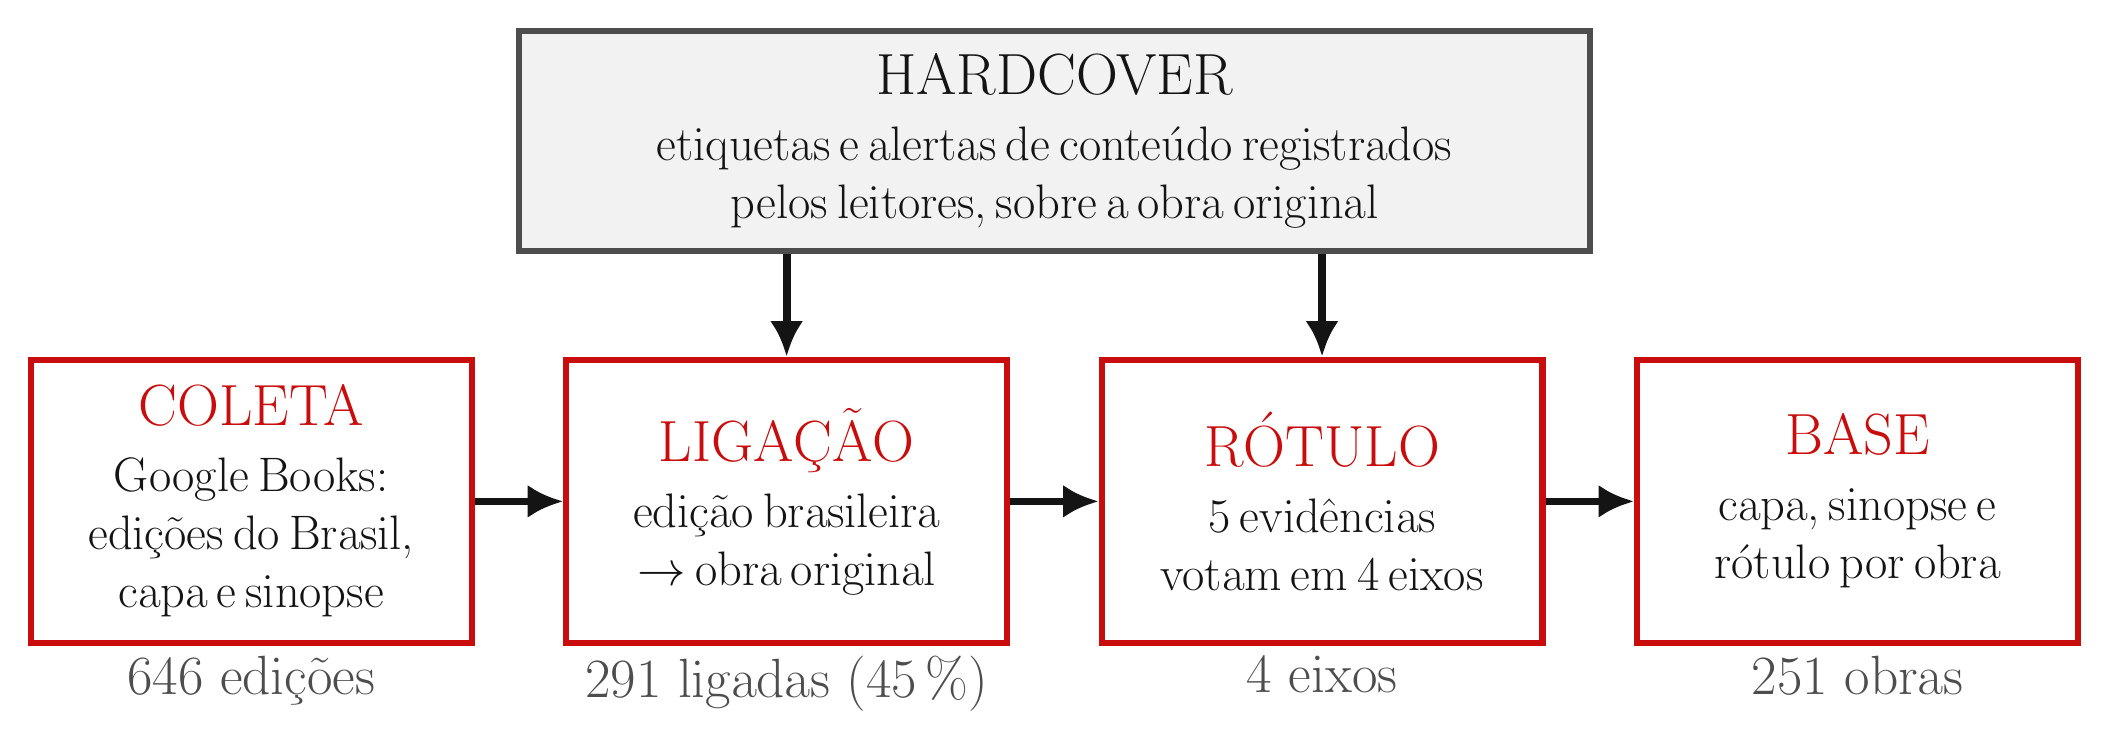
\begin{tikzpicture}[x=1cm, y=1cm,
      caixa/.style={draw=vermelho, line width=2.2pt, fill=white, text width=5.2cm,
        minimum height=3.6cm, align=center, inner sep=0.2cm},
      fonte/.style={draw=cinzaescuro, line width=2.2pt, fill=cinzaclaro, text width=13.0cm,
        align=center, inner sep=0.3cm},
      seta/.style={-{Latex[length=0.45cm,width=0.42cm]}, line width=2.8pt, preto},
      num/.style={font=\fontsize{20}{24}\selectfont\semib, text=cinzaescuro, anchor=north}]
    \node[caixa] (gb) at (0,0)    {\cx{COLETA}{Google Books:\\edições do Brasil,\\capa e sinopse}};
    \node[caixa] (po) at (6.8,0)  {\cx{LIGAÇÃO}{edição brasileira\\$\to$ obra original}};
    \node[caixa] (ro) at (13.6,0) {\cx{RÓTULO}{5 evidências\\votam em 4 eixos}};
    \node[caixa] (ba) at (20.4,0) {\cx{BASE}{capa, sinopse e\\rótulo por obra}};
    \coordinate (meio) at ($(po.north)!0.5!(ro.north)$);
    \node[fonte, anchor=south] (hc) at ($(meio)+(0,1.3)$)
      {\cx{\color{preto}HARDCOVER}{etiquetas e alertas de conteúdo registrados\\pelos leitores, sobre a obra original}};
    \draw[seta] (gb) -- (po);  \draw[seta] (po) -- (ro);  \draw[seta] (ro) -- (ba);
    \draw[seta] (hc.south -| po.north) -- (po.north);
    \draw[seta] (hc.south -| ro.north) -- (ro.north);
    \node[num] at (gb.south) {646 edições};
    \node[num] at (po.south) {291 ligadas (45\,\%)};
    \node[num] at (ro.south) {4 eixos};
    \node[num] at (ba.south) {251 obras};
  \end{tikzpicture}\par}
  \vspace{0.2cm}
  \etapa{LIGAÇÃO EDIÇÃO $\to$ OBRA}{Os leitores catalogam a obra original, não necessariamente a edição
    brasileira. A ligação é feita em cascata: ISBN, título, catálogo da autora e similaridade
    textual.}
  \etapa{RÓTULO POR EVIDÊNCIA CONVERGENTE}{Cinco evidências votam em quatro eixos: sexo,
    violência, abuso e drogas/álcool. Como livros pouco lidos recebem poucos alertas, a
    ausência de evidência resulta em \emph{indeterminado}, \textbf{nunca em \emph{baixo}}.}
\proxima

% ---------------- 3. resultados (parte 1): a base
  \secao{RESULTADOS: A BASE DE DADOS}
  \achado{1. A base reúne 251 obras de 49 editoras.}
  \vspace{-0.25cm}Distribuição do rótulo de conteúdo sensível:\par
  \begin{destaque}[top=0.45cm,bottom=0.3cm,left=0.8cm,right=0.7cm]
    \nivel{ALTO}{110}{evidência convergente}
    \nivel{PROV.\ BAIXO}{16}{sem evidência}
    \nivel{INDETERMINADO}{125}{evidência insuficiente: abstenção}
  \end{destaque}
  \vspace{0.45cm}
  {\pequeno\color{cinzaescuro}Prevalência de cada eixo nas 251 obras:\par}\vspace{0.2cm}
  \noindent\prev{35\,\%}{sexo / erotismo}%
  \prev{15\,\%}{violência}%
  \prev{15\,\%}{abuso / gatilhos}%
  \prev{7\,\%}{drogas / álcool}\par
\end{coluna}

% =====================================================================================
%  COLUNA DA DIREITA: Resultados (2 a 4) -> Conclusões -> Limitações e trabalhos futuros
% =====================================================================================
\begin{coluna}{30.8}
% ---------------- 4. resultados (parte 2): o que a base revela
  \secao{RESULTADOS: ANÁLISES}
% ---- resultado 2: omissão na sinopse
  \achado{2. A sinopse brasileira omite o tema em 68\,\% das obras com alerta de leitores
    (41 de 60).}
  {\centering
  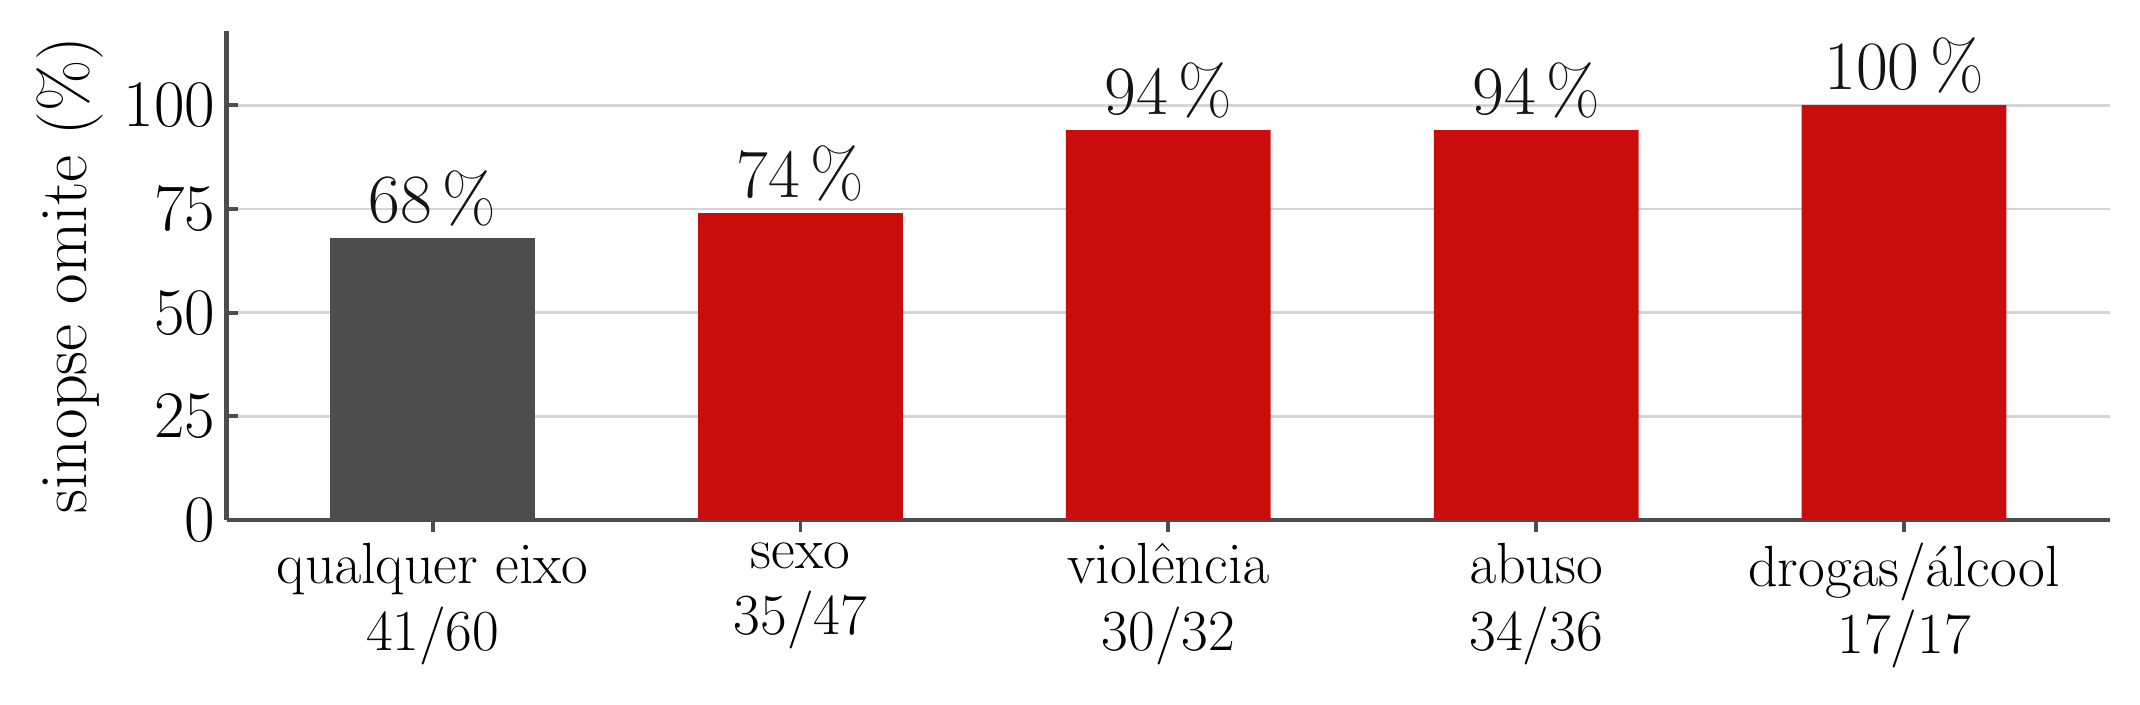
\begin{tikzpicture}
    \begin{axis}[ybar, bar width=2.6cm, width=25.5cm, height=7.8cm, ymin=0, ymax=118,
      enlarge x limits=0.14, symbolic x coords={q,sx,vi,ab,dr}, xtick={q,sx,vi,ab,dr},
      xticklabels={{qualquer eixo\\41/60},{sexo\\35/47},{violência\\30/32},{abuso\\34/36},{drogas/álcool\\17/17}},
      xticklabel style={align=center, font=\fontsize{21}{24}\selectfont},
      ylabel={sinopse omite (\%)}, ytick={0,25,50,75,100}, axis lines*=left,
      ymajorgrids, grid style={cinzamedio!40, line width=1pt},
      nodes near coords={\pgfmathprintnumber{\pgfplotspointmeta}\,\%},
      every node near coord/.append style={font=\fontsize{25}{29}\selectfont\semib, color=preto,
        /pgf/number format/fixed, /pgf/number format/precision=0}]
      \addplot[fill=cinzaescuro, draw=none, bar shift=0pt] coordinates {(q,68)};
      \addplot[fill=vermelho, draw=none, bar shift=0pt] coordinates {(sx,74) (vi,94) (ab,94) (dr,100)};
    \end{axis}
  \end{tikzpicture}\par}
  \vspace{0.1cm}{\pequeno\color{cinzaescuro}Obras cuja sinopse omite o
  tema / obras com alerta de leitores no eixo.\par}
\proxima

% ---- resultado 3: popularidade
  \achado{3. A informação disponível sobre uma obra cresce com a sua popularidade.}
  {\centering
  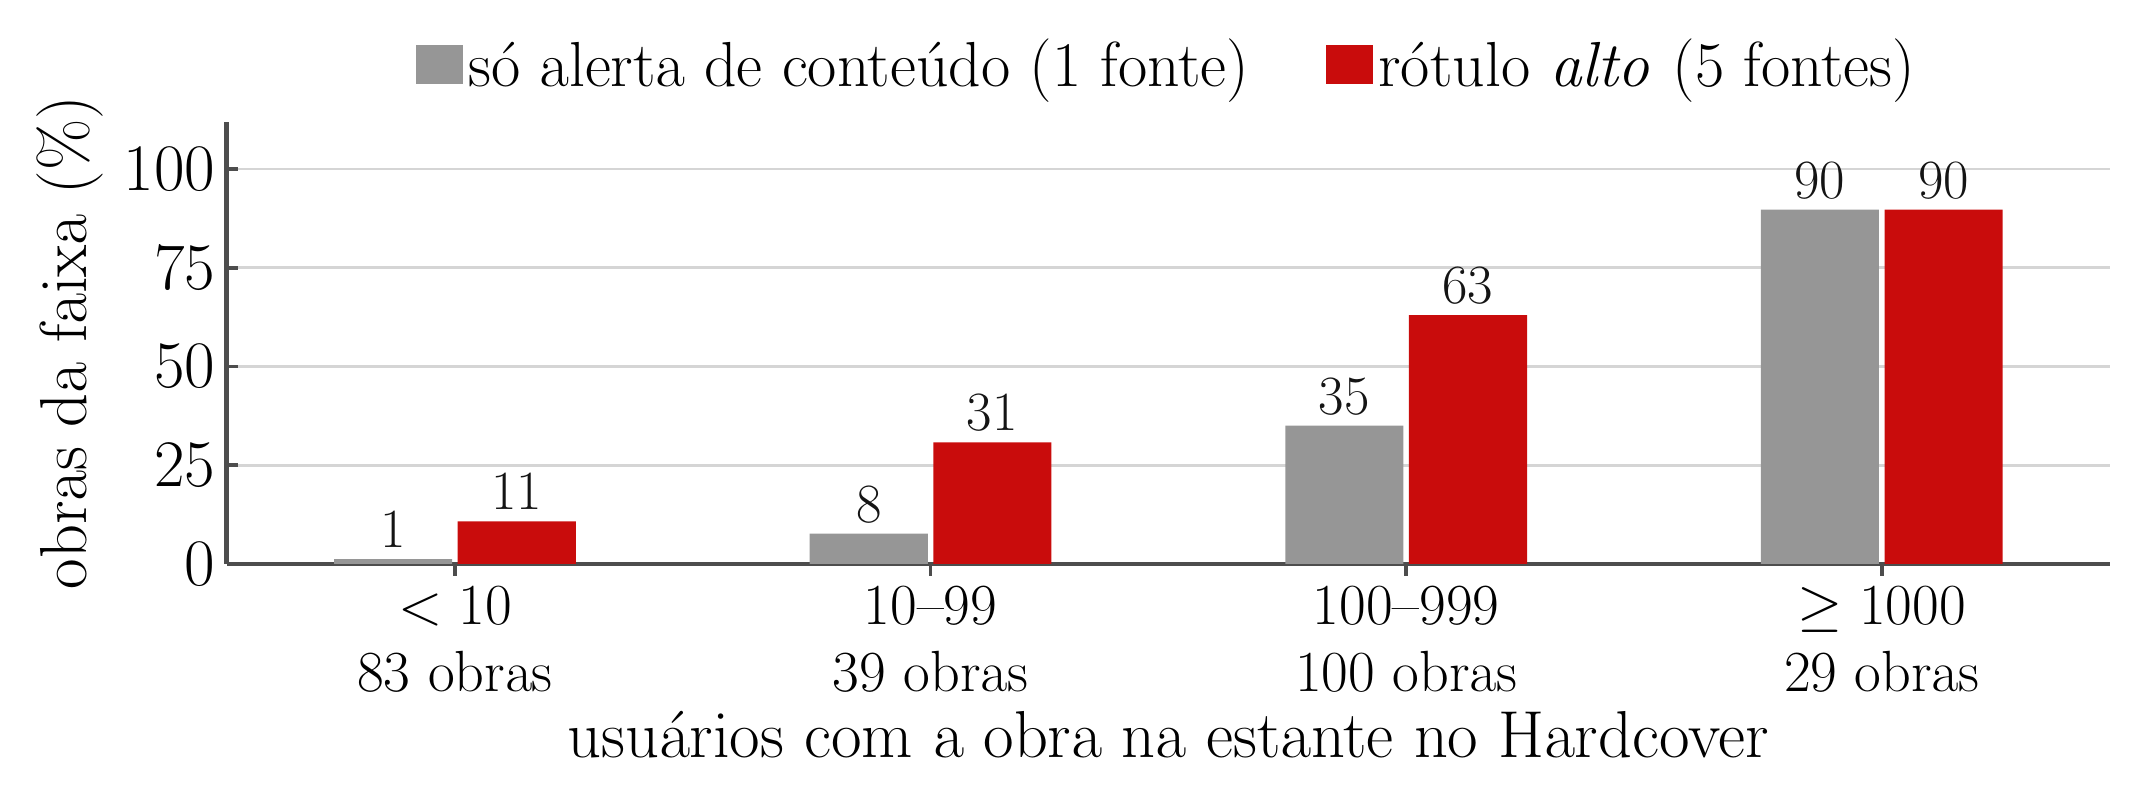
\begin{tikzpicture}
    \begin{axis}[ybar, bar width=1.5cm, width=25.5cm, height=7.2cm, ymin=0, ymax=112,
      enlarge x limits=0.16, symbolic x coords={a,b,c,d}, xtick={a,b,c,d},
      xticklabels={{$<10$\\83 obras},{10--99\\39 obras},{100--999\\100 obras},{$\geq 1000$\\29 obras}},
      xticklabel style={align=center, font=\fontsize{21}{24}\selectfont},
      xlabel={usuários com a obra na estante no Hardcover}, ylabel={obras da faixa (\%)},
      ytick={0,25,50,75,100}, axis lines*=left,
      ymajorgrids, grid style={cinzamedio!40, line width=1pt},
      legend style={at={(0.5,1.04)}, anchor=south, legend columns=2, legend cell align=left,
        /tikz/every even column/.append style={column sep=0.9cm}},
      legend image code/.code={\fill[#1] (0cm,-0.25cm) rectangle (0.6cm,0.25cm);},
      nodes near coords={\pgfmathprintnumber{\pgfplotspointmeta}},
      every node near coord/.append style={font=\fontsize{20}{24}\selectfont\semib, color=preto,
        /pgf/number format/fixed, /pgf/number format/precision=0}]
      \addplot[fill=cinzamedio, draw=none] coordinates {(a,1.2) (b,7.7) (c,35) (d,89.7)};
      \addplot[fill=vermelho, draw=none] coordinates {(a,10.8) (b,30.8) (c,63) (d,89.7)};
      \legend{só alerta de conteúdo (1 fonte), rótulo \emph{alto} (5 fontes)}
    \end{axis}
  \end{tikzpicture}\par}
  \vspace{0.1cm}
  De $<\!10$ a $\geq\!1000$ usuários na estante, os alertas sobem de 1\,\% para 90\,\%:
  \textbf{ausência de alerta não indica ausência de conteúdo}. Nas faixas médias, combinar as
  5 fontes já recupera obras ainda sem alerta.\par
\proxima

% ---- resultado 4: robustez (ablação). Fonte: outputs/tables/aval_ablacao.csv (todas as 9 linhas:
%      referência completo = 110 alto / 0 mudanças; 5 linhas "sem ..." e 3 linhas "so ...").
  \achado{4. Combinar as 5 fontes é necessário: todas ajudam e nenhuma basta sozinha.}
  {\centering
  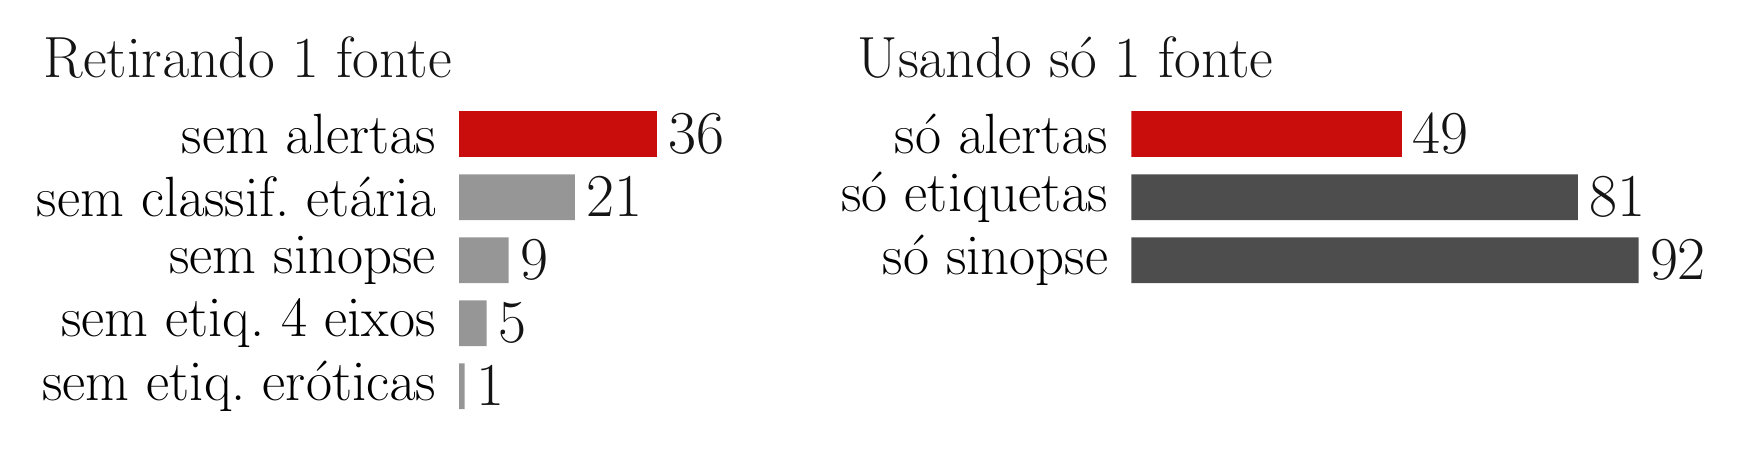
\begin{tikzpicture}
    \begin{axis}[name=esq, xbar, bar width=0.58cm, scale only axis, width=3.64cm, height=4.16cm,
      xmin=0, xmax=52, y dir=reverse, enlarge y limits=0.15,
      symbolic y coords={cw,ma,si,vo,ta}, ytick={cw,ma,si,vo,ta},
      yticklabels={sem alertas, sem classif.\ etária, sem sinopse, sem etiq.\ 4 eixos, sem etiq.\ eróticas},
      yticklabel style={font=\fontsize{20.5}{24}\selectfont},
      xtick=\empty, axis x line=none, axis y line*=left, axis line style={draw=none},
      ytick style={draw=none},
      nodes near coords, every node near coord/.append style={font=\fontsize{22}{26}\selectfont\semib,
        color=preto, /pgf/number format/fixed, /pgf/number format/precision=0}]
      \addplot[fill=vermelho, draw=none, bar shift=0pt] coordinates {(36,cw)};
      \addplot[fill=cinzamedio, draw=none, bar shift=0pt] coordinates {(21,ma) (9,si) (5,vo) (1,ta)};
    \end{axis}
    \begin{axis}[name=dir, at={(esq.north east)}, xshift=4.9cm, anchor=north west,
      xbar, bar width=0.58cm, scale only axis, width=7.70cm, height=2.56cm,
      xmin=0, xmax=110, y dir=reverse, enlarge y limits=0.30,
      symbolic y coords={scw,sco,ssi}, ytick={scw,sco,ssi},
      yticklabels={só alertas, só etiquetas, só sinopse},
      yticklabel style={font=\fontsize{20.5}{24}\selectfont},
      xtick=\empty, axis x line=none, axis y line*=left, axis line style={draw=none},
      ytick style={draw=none},
      nodes near coords, every node near coord/.append style={font=\fontsize{22}{26}\selectfont\semib,
        color=preto, /pgf/number format/fixed, /pgf/number format/precision=0}]
      \addplot[fill=vermelho, draw=none, bar shift=0pt] coordinates {(49,scw)};
      \addplot[fill=cinzaescuro, draw=none, bar shift=0pt] coordinates {(81,sco) (92,ssi)};
    \end{axis}
    \node[anchor=south west, font=\semib\fontsize{21}{24}\selectfont, text=preto]
      at ($(esq.north west)+(-5.4cm,0.12cm)$) {Retirando 1 fonte};
    \node[anchor=south west, font=\semib\fontsize{21}{24}\selectfont, text=preto]
      at ($(dir.north west)+(-3.6cm,0.12cm)$) {Usando só 1 fonte};
  \end{tikzpicture}\par}
  \vspace{0.1cm}{\pequeno\color{cinzaescuro}Obras (de 251) que mudam de rótulo frente ao
  modelo completo (5 fontes = 110 \emph{alto}): retirar uma fonte altera até 36 obras; usar
  uma só altera de 49 a 92.\par}
\proxima

% ---------------- 5. conclusões
  \secao{CONCLUSÕES}
  \begin{itemize}
    \item A base reúne, para \textbf{251 obras}, capa, sinopse e um rótulo independente da
      editora, que distingue \enquote{não tem} de \enquote{não sabemos}; é
      \textbf{reutilizável} e viabiliza o estudo de capa~$\times$~conteúdo.
    \item A sinopse \textbf{não é fonte confiável} do conteúdo: omite a maior parte dos
      temas que os leitores sinalizam.
    \item A popularidade deve ser \textbf{variável de controle} nesses estudos.
  \end{itemize}
\proxima

% ---------------- 6. limitações e trabalhos futuros
  \secao{LIMITAÇÕES E TRABALHOS FUTUROS}
  O rótulo detecta presença de evidência, nunca ausência; o vocabulário dos eixos é uma
  escolha; e só 45\,\% das edições coletadas foram ligadas a uma obra. \textbf{Próxima
  etapa:} comparar a estética das capas com o conteúdo, controlando a popularidade.\par
\end{coluna}

% ---------------------------------------------------------------- referências (rodapé)
\begin{bloco}{18.6}{17.9}{80.0}
  {\fontsize{15}{18}\selectfont\color{cinzaescuro}
  [1] IFLA. \emph{Functional Requirements for Bibliographic Records} (FRBR), 1998.\par
  [2] Christen. \emph{Data Matching}. Springer, 2012.\par
  [3] Ratner et al. Snorkel: rapid training data creation with weak supervision. VLDB, 2017.\par
  [4] Bekker e Davis. Learning from positive and unlabeled data: a survey. \emph{Mach. Learn.}, 2020.\par
  [5] Little e Rubin. \emph{Statistical Analysis with Missing Data}. Wiley, 2019.\par
  [6] Brasil. Lei nº 15.211/2025 (Estatuto Digital da Criança e do Adolescente).\par}
\end{bloco}

\end{document}
